\documentclass[12pt]{beamer}
\beamertemplatenavigationsymbolsempty

\usetheme{Copenhagen}
\useoutertheme{infolines}

\usepackage[utf8]{inputenc}
\usepackage[ngerman]{babel}
\usepackage{graphicx}
\usepackage{subfigure}
\title{Task 2 -- Parkassistent}
\institute{EvoTest}
\author{Alex, Yaroslav, Manuel}
\date{16.11.2016}

\begin{document}
\maketitle 

% here another input

\section{Algorithmus}
\begin{frame}{Algortihmus}

\begin{enumerate}
	\item Bereche den Zielpunkt
	\item Wenn es zwei Spurkreise gibt, die sinnvoll am Zielpunkt und am Ausgangspunkt anliegen und sich berühren
  \begin{enumerate}
		\item Erstelle aus diesen Spurkreisen Steuersignale \label{Signale}
		\item Terminiere
	\end{enumerate}
	\item Andernfalls berechne einen Punkt außerhalb der Parklücke, von dem aus \ref{Signale} erreichbar ist und der außerdem nur eine einzige Begrenzung neben sich hat.
	\item Steuere diesen Punkt mittels einer leicht veränderten Variante des Models von Dubin's Car an und terminiere. 
\end{enumerate}

\end{frame}
\subsection{Zielpunkt Berechnen}
\begin{frame}{Zielpunkt Berechnen}
	Idee: Wähle einen Punkt, von dem man möglichst leicht in einem Zug einparken kann.
	
	\begin{columns}
		\begin{column}{0.5\textwidth}
			\begin{figure}
				\centering
				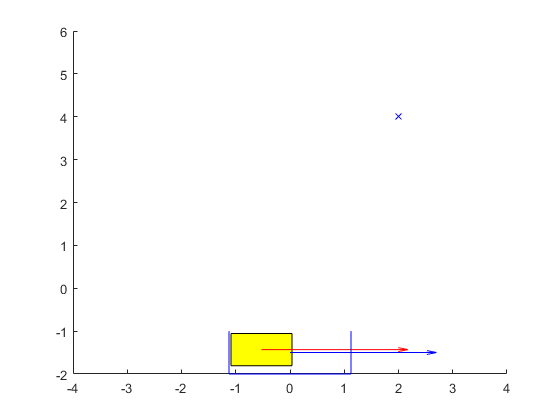
\includegraphics[width=\textwidth]{images/ex2step1example1.png}
			\end{figure}
		\end{column}
		\begin{column}{0.5\textwidth}
			\begin{figure}
				\centering
				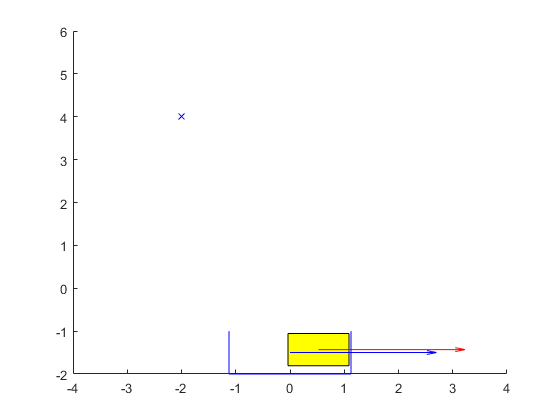
\includegraphics[width=\textwidth]{images/ex2step1example2.png}
			\end{figure}
		\end{column}
	\end{columns}
	
\end{frame}
\subsection{Direktes Einparken}
\begin{frame}{Einparken in einem Zug}
Idee: Parke direkt in einem Zug ein durch nur eine Rechtslenkung und eine Linkslenkung.

	\begin{columns}
		\begin{column}{0.5\textwidth}
			\begin{figure}
				\centering
				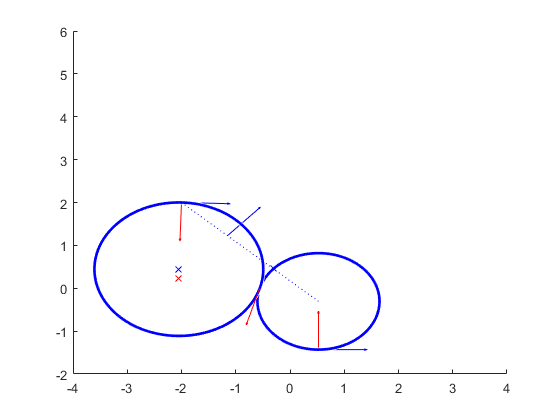
\includegraphics[width=\textwidth]{images/ex2step3example1.png}
			\end{figure}
		\end{column}
		\begin{column}{0.5\textwidth}
			\begin{figure}
				\centering
				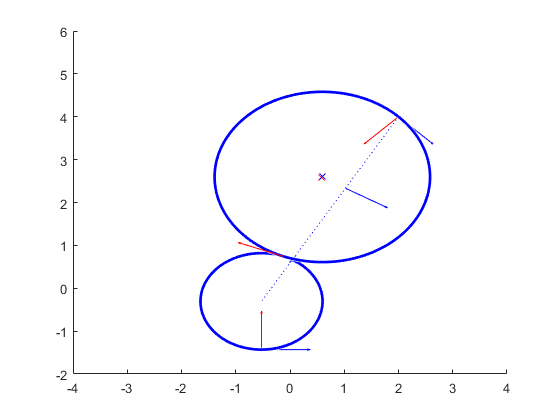
\includegraphics[width=\textwidth]{images/ex2step3example2.png}
			\end{figure}
		\end{column}
	\end{columns}
\end{frame}
\subsection{Dubin's Car Vorbereitung}
\begin{frame}{Vorbereitung für Dubin's Car}
	Idee: Nimm denselben Zielkreis wie in Schritt 3 und fahre ihn von einer Position außerhalb des Parkplatzes an.
	
	
	\begin{figure}
		\centering
			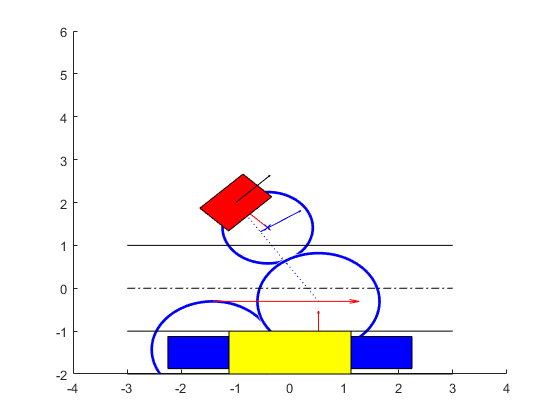
\includegraphics[width=0.75\textwidth]{C:/Users/Alexander/EvoTest/doku/task2/images/ex2step4example.png}
		\label{fig:ex2step4example}
	\end{figure}
	
\end{frame}

\section{Steuersignalerzeugung}
\begin{frame}{Steuersignalerzeugung}
Im Anschluss an die Geometrieermittlung folgt die Berechnung der Steuersignale.

Es existieren zwei primitive:
\begin{itemize}
\item Gerade
\item Kreise
\end{itemize}
Beide sind in Klassen gekapselt, die Schnittstelle
\[ctrl\_signal = calcCtrlSignal(velocity,\,axis\_length)\]
dient dann der Erzeugung des Kontrollvektors:
\[[velocity\,steering\_angle\,duration]\]
\end{frame}

\subsection{Geraden}
\begin{frame}{Steuersignale -- Geraden}
Für geraden ist die Steuersignalerzeugung trivial:
\begin{itemize}
\item Der Lenkwinkel ist Null
\item Die Dauer des Steuersignals ist abhängig von der zurückzulegenden Entfernung $x$ und der Geschwindigkeit $v$. Aus $v=\frac{s}{t}$ abgeleitet werden: $t=\frac{s}{v}$
\end{itemize}
Die Geschwindigkeit entspricht der gewünschten Geschwindigkeit.
\end{frame}

\subsection{Kreise}
\begin{frame}{Steuersignalerzeugung -- Kreise}
Kreise sind komplexer:
\begin{itemize}
\item Der Lenkwinkel hängt von der Krümmung des Kreises und damit von dessen Radius sowie dem Achsabstand ab:  $atan(achsabstand/radius)$
\item Die Dauer hängt von der Wunschgeschwindigkeit und der Länge des Kreissegments ab: \[\frac{Winkelsumme\cdot Radius}{Geschwindigkeit}\]
\end{itemize}
Die Geschwindigkeit entspricht der gewünschten Geschwindigkeit.
\end{frame}

\end{document}